\chapter{NDT graph-SLAM overview}
In this chapter we will present our solution to create 2D varian of graph based \gls{SLAM} on \gls{NDT} maps. This chapter starts with complete overview of algorithm. In next sections we explain how we have designed each part of the system.
\section{System composition}
\label{sec:Sys_arch}

Standard input of many \gls{SLAM} algorithms is odometry. In our case we do not require any prior information about robot movements. Robot position estimation is done by fast incremental scan matching. The only mandatory input is a point cloud extracted from robot's measurement. Scan matcher calculates relative transformation based on received point cloud and incremental scan matcher's map. We will refer to this map as to the moving window. It is created by merging multiple old point clouds. More details will be provided in section \ref{sec:window}.

Resulting transformation is used in the \gls{NDT} frame creation process. \gls{NDT} frame is small map which is created out of couple consecutive scans. Precise transformation is used to correctly merge these scans into single frame. This mini map is than used as a measurement information in a node of pose graph. Creating small \gls{NDT} frames solves problem measurements with small number of points. Imagine situation where robot is standing close to the corner of the room. In this scenario incoming point clouds hold only small number of points, because field of view is narrow. Similar problem arise if robot uses sensor with limited field of view e.g. Kinect. To solve it we need to integrate multiple scans to get better outline of the world. More information about world also helps to reduce chance of ambiguous loop detections \ref{sec:Scan_reg} because larger frames have higher chance to include more unique features. Additionally, we also want to utilize advantages of \gls{NDT-OM} occupancy update rule. It is able to detect dynamic objects by ray-tracing and update map accordingly. This detection is done by merging multiple scans and re-observing same cell multiple times. More information about design choices behind \gls{NDT} frames are in section \ref{sec:NDT_frame}.

After \gls{NDT} frame generation phase, algorithms creates representing node in pose graph. Each two nodes are connected by odometry edge. Original odometry received from scan matching process was used to create \gls{NDT} frames. In our abstraction, odometry is represented by transformation between origins of consecutive frames. In the next step, pose graph generates possible loop closure edges. To do so we need to traverse a graph with use of Dijkstra projection and apply our radius based metric described in section \ref{sec:LoopClosureMetric}. 

The potential matches need to be robustly aligned. Solution to this problem is the most difficult. We need algorithm which is able to perform 10s of registration per second. At the same time it needs to reject matches which are not from the same part of the environment. In addition, some errors caused by local and global ambiguities \ref{sec:Scan_reg} are very difficult to avoid. We propose solution to these problems by improving version of \gls{D2D}-\gls{NDT}. In this adaptation, we utilize robust initial pose estimation from Correlative scan registration \ref{subsec:Corr} and for finer alignment \gls{D2D}-\gls{NDT} \ref{subsec:D2D_NDT}. Full description is provided in \ref{sec:Robust D2D-NDT}.

Generated loop closure edges needs to be validated against possible outliers. In this matter we have decided to use robust optimization engine with switchable constrains. We have made decision based on comparative study by \cite{RobustOpt}, where this method offered the best result in comparison to execution time. We need to minimize amount of time spent in optimization. Saved time can be used to validate more loop closure edges. Second important factor in optimization process is number of nodes and edges in graph. Computation time grows with increasing number of elements in the graph. We are limiting number of nodes by using \gls{NDT} frames. Frames can be farther away from each other, because they accumulate multiple measurements.

Smaller number of nodes in graph also mean less work to \gls{NDT} mapper. In case of successful loop closure we need to regenerate map based on new position of nodes in graph. In this version of algorithm we just simple iterate over all frames and merge them to the new map based on new origins. In the future \gls{NDT} frames allow to only generate part of the map based on request from user. It could also be possible to dynamically load and save individual frames based on their need and save memory for long run of algorithm.

Combining these parts together creates whole graph base \gls{SLAM} algorithm on NDT maps.   

\begin{figure}
	\centering
	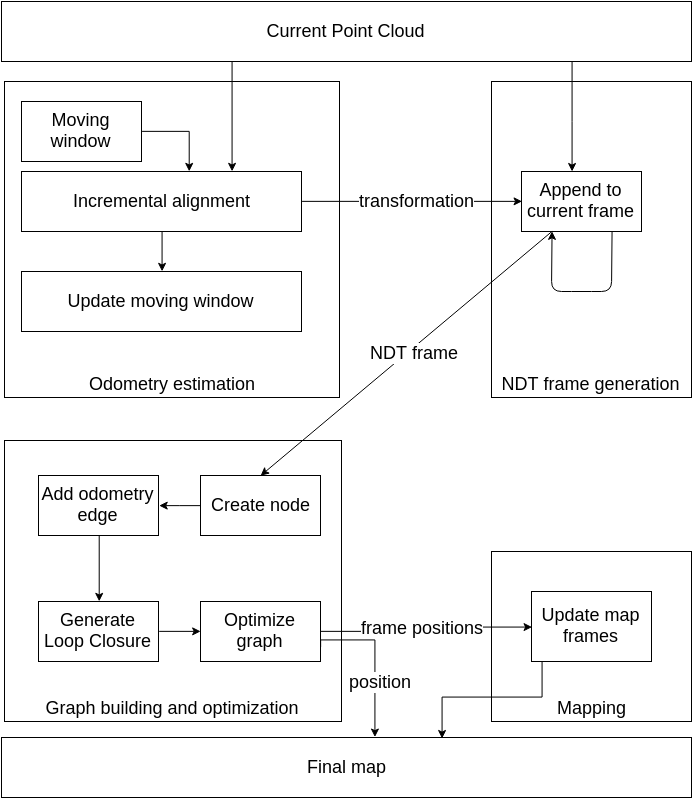
\includegraphics[width=100mm]{../img/algorithm_runtime.png}
	\caption{Diagram of graph based SLAM on NDT maps}
	\label{fig:algorithm}
\end{figure}
  
\newpage


\section{Moving window}
\label{sec:window}
Moving window is a special type of \gls{NDT} grid. It uses all features of \gls{NDT-OM} including occupancy update and dynamic object rejection. Main idea behind moving window is to offer small map which can be used by incremental scanmatcher in order to efficiently align incoming scans against longer history. In standard incremental scanmatching approaches we need to know whole map. Information from whole map is used to correct small errors  when revisiting same place. A problem with this method arise when alignment fails. In this case wrongly aligned scan is merged into the map. This creates single environment feature multiple times in the map. This can be wrongly understood by next registration and error might be never corrected. \gls{NDT-OM} can solve some of degeneration be cleaning occupied cells which are on the way between robot position and new measurement. In order for this mechanism to work next alignment scan needs to converge to original correct position. This is very unlikely with already corrupted mapmand standard NDT technics for registrations, which can end up in local optima during scan refinement step.

In our system, we do not need to know whole map of environment because loops closures errors are fixed by graph optimization. We need incremental scanmatcher to provide us good local estimate of robot movement. For this purpose we only need to know the part of environment occupied by current scan. It strongly depends on the type of sensor and environment. In our setup, robot operated in indoor environment with laser sensor ranging up to 20m in long corridors. In this scenario window size of 20m should incorporate all information which can help in scan registration. If it is possible to select smaller window size based on environment structure this adds to additional speed  and memory efficiency. 

The mowing window also needs to follow movement of the robot to incorporate new measurements. This can be done in two ways. First we might rotate window based on exact changes of robot global position. By doing this we need to transfer whole window  after each small movement of robot. This approach tries to transform every single normal distribution inside grid in every step of algorithm. Transformed cell's distribution may suddenly overlap multiple fields. We would need to develop mechanism how to split original distributions into multiple cells. Better way is to keep windows orientation fixed and only translate window based on robot's movement. This prevents rotation of distributions in cells, but still suffer from same spiting problem. Solution to this problem is by moving window only in multiples of the grid. This does not affect parameters of normal distribution inside of original grid in order to move whole window. After movement some cells may get out of the scope of current window. These cells are destroyed. This also helps to reduce accumulated error in the window by deleting old corrupted measurement. 

To minimize any alignment issues we decided to perform fast scan matching. This means process most of the data from laser. High frequency scan matching does not need initial guess because valid result is reasonably close to inital position of source and target measurements. Registration algorithm capable of this performance needs to work in order of milliseconds. Two algorithms developed for fine registration on top of \gls{NDT} grid are \gls{P2D}-\gls{NDT} and \gls{D2D}-\gls{NDT}. We have decided to use standard \gls{D2D} algorithm, because it offers ten times better run time than \gls{P2D}. Comparative study by \cite{NDTcomparative} shows that even though \gls{P2D} is usually more precise it needs significantly more computation time. Skipping multiple measurements from sensor may cause that we will not be able to robustly estimate transformation and whole process can converge to local minimum. 

\begin{algorithm}
\label{alg:move_window}
    \caption{Moving window processing loop}
\begin{algorithmic}[1]
\Require point cloud $X$, move window's \gls{NDT} grid $M$, transformation $T_{o}$ to the origin of moving window, transformation $T_{r}$ unused from move in last call of function, transformation $P$  last known absolute pose of moving window.  
 \Function{calculateTransform}{$X$}
	 \State $X_{o} \gets$ transformPointCloud($X$,$T_{o} * T_{r}$)
	 \State $N_{o} \gets$ createNDTGrid($X_{o}$)
	 \State $T_{ox} \gets$ alignD2D($N_{o}$,$M$)
	 \State $M$.mergeIn($X_{o}$,$T_{ox}$)
	 \Comment applies transformation on point cloud and merge it into moving window
	 \State $T_{diff} \gets P^{-1} * (T_{o} * T_{ox})$
	 \State $P \gets T_{o} * T_{ox}$
	 \Comment update of absolute pose of window for next call 
	 \State $T_{r} \gets M$.moveWindow($T_{ox}$)
	 \State \Return $T_{diff}$
 \EndFunction
\end{algorithmic}
\end{algorithm}
\todo{add visualization of running window}

\newpage

\section{NDT frame creation}
\label{sec:NDT_frame}
\gls{NDT} frame is created by merging multiple point clouds based on transformation received from odometry estimation. Important question is how many scans should we combine ? This algorithm uses consecutive addition of transformation as in equation \ref{eq:concat_trans}. Afterwards, it calculates total displacement done by robot. If it is more than threshold we close down old \gls{NDT} frame and start to add scans into new empty frame. A new frame is assigned its coordinate system based on current robot position. Every new scan is transformed into coordinate system of current open frame and merged in. Closed frame is sent to pose graph generation where it is transformed into graph's node.

Selection of good displacement value is important for run of whole algorithm. Small value will create many nodes in pose graph. Every node will reflect only small portion of environment. This will make loop closure computationally expensive by need to evaluate too many possible loop closure nodes. At the same time loop closing algorithm will work with only limited information. This may cause bigger number of local and global ambiguities in registration. A large value of displacement will generate fewer nodes with more information in each node. This is less computationally dependent. On the other hand it creates ambiguous environment inside of \gls{NDT} frame. Loop closure registration may not correctly deduct which part of the same environment in the frame is correct for registering. This forces registration algorithm to correctly identify this situation and solve it. At the same, it wastes optimizer potential for rejection of ambiguous alignments based on topological information of whole environment. 

\section{Loop closure detection}
\label{sec:LoopClosureMetric}
Loop closure detection is done on top of pose graph. Loop detector can use current positions of pose graph's nodes and relative transformations stored in odometry and loop closure edges. With this information we need to find all nodes which can with current node create loop closure edge. The process starts by Dijkstra projection in section \ref{subsec:loop_closure_creation} from current node. During this process algorithm also  calculates relative displacement along edges. Sum of displacements is used as parameter for rejection of nodes which are too close to our current position. These nodes are certainly overlapping with our start node and therefore it is not necessary to check them again. All the nodes passing previous test are used in one of two rejection models. 

First model tests all nodes against selected radius. Second mechanism is using cumulative transformation and covariance calculated by Dijkstra projection. In validating if two nodes overlap we use same metric as presented by \cite{Olson2009Loop}.
\begin{equation}
\varDelta c = (c_{b} - c_{a})
\end{equation}
\begin{equation}
s  = \max(0,\lVert \varDelta c\rVert - r_{a} - r_{b})\frac{\varDelta c}{\lVert \varDelta c\rVert}
\end{equation}
\begin{equation}
mahl = s^{T}P_{a,b}^{-1}s
\end{equation}
where $c_{a}$ and $c_{b}$ are centroids of start and currently compared \gls{NDT} grids; $r_{a}$ and $r_{b}$ are radii of respective \gls{NDT} grids and $P_{a,b}^{-1}$ is inverse of accumulated covariance.
 
Selected nodes are registered by robust \gls{D2D}. Those matches with high score are inserted into the graph. Edges added by this mechanism may still include some errors or ambiguities. Rejection of these edges is done in optimizer.


\section{Robust D2D-NDT registration}
\label{sec:Robust D2D-NDT}
Construction of robust \gls{D2D} registration needs to be fast and precise. In addition, it needs to have a mechanism how to reject invalid association. It also needs to use only information present in \gls{NDT} grids because loop closure mechanism is working only with this data. We knew that \gls{D2D} can offer quick a reliable registration on \gls{NDT} grids with good initial guess. Correlative scan matching algorithm  \ref{subsec:Corr} can provide registration without knowledge of initial guess but in standard version is not possible to operate on top of \gls{NDT} grids. The time performance of this algorithm is also slower than \gls{D2D}. To solve these problems we have developed modified version of correlative algorithm which can work on top of \gls{NDT} grids.

\subsection{Adaptation of correlative registration}
We have started with base algorithm described in section \ref{subsec:Corr}. For our needs it is sufficient when this algorithm provides only rough initial guess. For this reason we use only one layer architecture. Our single grid has cell size double of original size of \gls{NDT} grid. One reason is faster execution time. In first part of algorithm we need to go over large search space. Mainly because we cannot expect any prior information from graph. Larger grid size limits number of translation because we always try translations in multiple of cell size as mentioned in \ref{subsec:Corr}. 

Secondly, we need to transfer original \gls{NDT} grid into reasonable point cloud. In our implementation we have decided to recreate point cloud out of grid by taking mean from every cell with distribution. Colection of these means makes our mean cloud. In addition, we use information about how many points were used to create normal distribution. This information is used in our algorithm as weight for every mean value. Original algorithm uses two point clouds. 

First is called target cloud and is used for creation of look up table. This table is created by projecting all points to individual cells. When is cell occupied by at least one point it is marked with value 1. In our scenario we use cloud of means from target grid to construct look up table. Use of means is more robust to outliers than original look up table from point cloud. Original implementation marked occupied every cell regardless on number of points mapped into it. Our grids needs at least 4 points to create normal distribution. This is limiting influence of single point spread in space and also emphasizing dominant structures in environment. Target grid conversion to mean cloud does not loose any information in comparison to original cloud. This is because look up table and traget grid are aligned. On top of that double step size of look up table makes four cells from target \gls{NDT} contribute to single look up cell.
  
Second source cloud is used for scoring on top of look up table. Every point of point-cloud contributes to total score based on value from look up cell it belongs to. In our case single point represents information about mean center of multiple points. In order to keep all information, algorithm maps mean into correct cell in look up table. By doing this mean only contributed once. Fortunately a score generated by mean can be scaled with use of weight associated with mean. This makes weighted mean point contribute same amount to system as standard points from point cloud. Score function is defined as:
\begin{equation}
score(T,C) = \frac{1}{d}\sum_{p \in C}^{} v(T,p) w(p) 
\end{equation}

where $T$ is transformation which should be applied to point $p$ of cloud $C$. A function $v(T,p)$ applies transformation $T$ to point $p$ maps it to look up table and return score value for single point. A function $w(p)$ return weight of current mean point. Scaling factor $d$ is defined as
\begin{equation}
d = m\sum_{p \in C_{t}}^{}w(p)
\end{equation} 
where $m$ is the maximal value one point can receive from look up table after application of smoothing kernel in equation \ref{eq:smooth_kernel}; $C_{t}$ represents target point cloud. 

Last problem with conversion of source cloud to mean cloud is to handle discretization errors. These errors happen when we need to transform \gls{NDT} grid. In this situation one original \gls{PDF} may overlap multiple cells. A original point cloud would contribute into multiple cells. Our mean formulation would contribute only to one cell based on mean location. To minimize this effect, we map every mean value into the taget look up table which has double cell size in comparison with source \gls{NDT}. This process is similar to multi layer discretization removal in multi layer \gls{NDT} registration \cite{ulas20113d}. Target look up table also include smoothing kernel, which assign some value to cells surrounding occupied cell in table. This also makes mean which could potentially slip out of occupied cell's boundaries contribute into the total score.

By executing these approximations, we were able to create version of correlative estimate on top of \gls{NDT} grids. Coarser resolution improved performance and allowed us search larger search space. Approximation of input cloud into means reduced number of point we need to test in every iteration of algorithm loop. This effectively lowered number of look up table calls, which speeds up whole process. In addition, mean cloud removes outliers from points spread in space.

\subsection{Algorithm overview}
With coarse initial guess estimate we can  constrict whole algorithm. First step is to run on pair of grids correlative estimation algorithm. This offers us the best initial guess it could find in selected search space. In this step we have used coarse look up table. This means that we are still possible almost two \gls{NDT} cell away from right solution. To get right alignment we run \gls{D2D} algorithm. Multi layer definition of \gls{D2D} can converge to right solution if there is one. Problem arise if two matched grids are from diffrent locations and do not share same environment features e.g lines, corners. In this case correlation registration finds the best possible solution, which means that it rotates grid in a way that maximalize score. \gls{D2D} than tryist to find best alignment and usually falss to first local minimum it can find. To solve these situations we propose solution validation process. Example of bad alignment is in figure \ref{fig:bad_align}. 



\subsection{Solution validation}
Robust alignment offers us the best transformation between source and target \gls{NDT} grid. This alignment can fail and do not offer successful registration at all. We need to validate if this registration succeeded or failed. In this algorithm we again use correlative scan matcher. In this case we use cell size of target look up table matching cell size of \gls{NDT} target grid. We map every point from mean source cloud into look up table and receive total score based on contributions of each weighted mean point. In this case discretization is helping us provide better results. In case that some means stay out of target grid it means that registration was less successful which result in lower score. This method is able to reject scans based on their overlap. This method is not able to distinguish wrong alignment in case that two scans look similar but originate in two different parts of environment.

\begin{algorithm}
\label{alg:robust_d2d}
    \caption{Robust \gls{D2D} registration algorithm}
\begin{algorithmic}[1]
\Require source \gls{NDT} grid $G_{s}$ and target \gls{NDT} grid $G_{t}$. Resolution of \gls{NDT} grids $r$. Validation threshold $v$
 \Function{align}{$G_{s}$, $G_{t}$, $r$}
 \State transformation T is identity
 \State ($T$,$score$) $\gets$ correlativeEstimater($G_{s}$, $G_{t}$,$T$, $2*r$)
 \State $T \gets$ alignD2D($G_{s}$, $G_{t}$,$T$)
 \State ($T$,$score$) $\gets$ correlativeEstimater($G_{s}$, $G_{t}$,$T$, $r$)
 \If{$score \geq v$}
	 \State \Return ($T$,$true$) 
 \Else
	 \State \Return ($T$,$false$)
 \EndIf
 \State \Return T 
 \EndFunction
\end{algorithmic}
\end{algorithm}

\begin{figure}
	\centering
	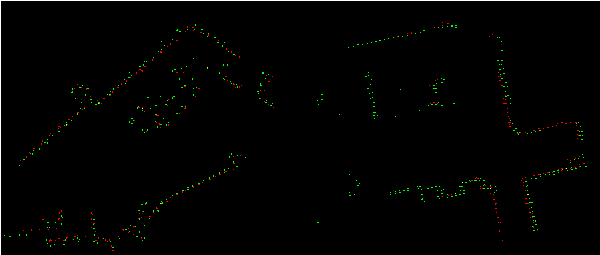
\includegraphics[width=150mm]{../img/good_align.png}
	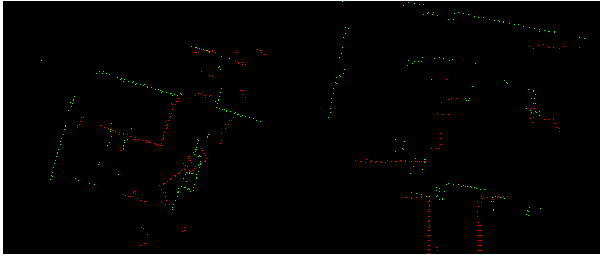
\includegraphics[width=150mm]{../img/bad_align.png}
	\caption{Images with alignment. Red dost represent target scan and green dots source scan. The first row shows valid alignment marked with high score. Second row shows two alignments which were rejected by validation.}
	\label{fig:bad_align}
\end{figure}
\newpage
